\chapter{Computational Models for Disordered nanowire networks}
%The aim of this chapter is to introduce the computational framework to numerically calculate the sheet resistance of a nanowire network where inner wire resistance is both included and excluded. A method to digitise SEM images of nanowire networks is presented allowing for simulations on a near identical network connectivity with physical networks whose resistance has been experimentally measured. The digitised network geometry and the inclusion of nanowire resistance allows us to estimate the inter-wire junction resistance and it is shown to agree closely with experimental measurements. A method to determine the ultimate conductivity of a nanowire network, i.e. where inter-wire junctions are perfect conductors, is presented and applied to several experimental samples. Aspects of theis work have been published in ...
%\newpage
%\section{Chapter Motivation}
The conductance of a nanowire network depends on a multitude of underlying parameters: the length and diameter distributions of nanowires\cite{hecht2006,bergin2012,sorel2012,hicks2009,pike1974}, inter-wire junction resistances\cite{mutiso2013}, resistance of nanowire segments{\cite{zezelj2012}, wire density\cite{balberg1983}}, connectivity profile, and device dimensions\cite{fairfield2014} to name but a few. All of these parameters and physical features will impact the conductance of a NWN. A common method of numerically solving this complex transport problem\cite{kirkpatrick1973} is to map the NWN onto a node-voltage graphical representation where each nanowire is a node in the graph and is connected to its nearest neighbours by a resistor corresponding to the inter-wire junction. Kirchhoff's circuit laws and Ohm's law are applied to the node-voltage graph to calculate the conductance of the system as outlined in chapter 2\cite{graph_book}. An implicit assumption is being made in this approach: the junction resistance is much higher than the nanowire inner resistance and so dominate the electrical properties of the network. This approach shall be referred to as the Junction Dominated Assumption (JDA) henceforth. 
%With such a large parameter space determining a relationship between the conductance of a NWN and the underlying parameters is difficult, requiring fitting of empirical functions to the results of large scale Monte Carlo simulations.

Monte Carlo simulations of conductive stick networks show that their electrical properties are highly sensitive to the ratio $R_{in}/R_{j}$, where $R_j$ is the resistance of a junction and $R_{in}$ is the inner resistance of a wire segment\cite{li2009,hicks2009,zezelj2012}. The JDA model has successfully calculated the resistive properties of carbon nanotube networks, as the nanotube resistance is negligible compared with the resistance of a nanotube junction\cite{nirmalraj2009,hecht2006}. Metallic nanowire junctions however have been shown to have relatively low junction resistances\cite{bellew2015} and, as a result, the nanowires themselves have a sizable impact on the network conductivity. With the demand for increasing NWN conductivity for optoelectric device applications\cite{bellet2017,gong2017,langley2013}, $R_j$ is continuously being minimised by effective annealing techniques\cite{madaria2010,hwang2014,liangbing2010,nirmalraj2012} and so the JDA is not appropriate for these systems. In this chapter, we introduce a model that includes both nanowire resistances ($R_{in}$ and $R_j$), the Multi-Nodal Representation (MNR), and show how both MNR and JDA models depend differently on the underlying parameters mentioned at the start of the chapter.

A fundamental issue with nanowire network simulations is the inherent spatial randomness of wire positions and their impact on network connectivity. Experimental measurements can only be related to the average results of simulations with matching underlying parameters in order to obtain meaningful results\cite{mutiso2013}. To directly compare computational simulation with experimental measurements, we developed a method to digitally capture the positions and orientations of nanowires from Scanning Electron Microscope (SEM) images of NWNs. The goal of this chapter is to compare MNR and JDA simulations using both configurational averaging and digitised networks from experimental samples to understand the effect of nanowire resistance on certain network properties.

The layout of this chapter is as follows. In section \ref{sec:Graphical Representations of NWNs}, the JDA and MNR models are presented and the computational simulations are outlined. In section \ref{Sec: Resistive properties}, MNR and JDA approaches are applied to simulations of NWNs and the dependence of sheet resistance on a selection of nanowire properties are explored, highlighting the impact of inner-wire resistance on these relationships. In section \ref{sec:image_proc}, an original technique that digitises images of experimental NWNs is introduced to which the JDA and MNR are applied. The digitised networks can be used to approximate the junction resistance of the samples and these results were compared with a distribution of junction resistances that were measured experimentally\cite{bellew2015}. The ultimate conductivity of a NWN, which can be obtained when junctions are annealed to their optimum capacities, is then calculated for each of the experimental samples. A novel way of quantifying the potential for network conductance improvement is introduced in section \ref{sec:image_proc} and its dependence on several network parameters is presented\cite{rocha2015}. In section \ref{Sec: Dispersion}, the effect of including dispersion in the junction resistances is examined for MNR and JDA mappings. A short chapter summary is presented in section \ref{sec:Conclusion}.
%==================================================
\section{Graphical Representations of Nanowire Networks}
\label{sec:Graphical Representations of NWNs}

To calculate the resistive properties of a NWN, the nanowire mesh must be mapped into a mathematical graph that captures the connectivity information of the network to which node-voltage points are assigned. In this way, Kirchhoff's system of linear equations introduced in chapter 2 can be used. In the JDA mapping, each wire is represented by a circuit node at a common voltage connected to other wires by junction resistors (edges of the graph). A NWN with $N_w$ wires will result in a resistive graph with $N_w$ nodes. An off-diagonal element in the Kirchhoff matrix ($K^{jda}_{ij}$) is the conductance of the inter-wire junction between wires $i$ and $j$. Figure \ref{fig: mnr_jda_sketch}(a) is a sketch of a simple NWN (top) with its JDA graphical representation (bottom). There are three nodes in this graphical representation, one for each nanowire, and two inter-wire junctions with resistance $R_j$. Note that there is no junction between wires $W_1$ and $W_2$, thus there is no resistor for this connection in the graph representation. The locations of the nanowires are irrelevant in the JDA; only the connectivity profile of the network and $R_j$ determine its electrical properties. As this mapping only acts on the inter-wire connectivity, the inner-wire resistances of the nanowire segments are entirely omitted from this model.

\fig{1.0}
{Images/Chapter3/mnr_jda_sketch_lowQ.png}
{\textbf{Schematic:} Mapping a nanowire network with JDA and MNR models.}
{ (a) A sketch of a simple NWN with three wires labeled $W_i$, $i = 1,2,3$ and two inter-wire junctions, one between wires $W_1$ and $W_2$ and another between wires $W_1$ and $W_3$\cite{rocha2015}. Underneath the sketch is a circuit representation of the NWN; there are three nodes corresponding to the three wires and two inter-wire junction resistors represented by black resistors with resistances $R_j$. (b) An expanded view of the three wires sketched in panel (a). The four connection nodes, two for each inter-wire junction, are shown as the red dots labeled $C_i, ~ i=1,2,3,4$. Underneath the sketch is an MNR circuit representation of the NWN. Connection nodes associated with the same junction are connected by a junction resistor $R_j$ and shown in black. The connection nodes that are adjacent on $W_3$, $C_2$ and $C_4$, are connected by a nanowire segment resistor $R_{in}$ illustrated by the yellow resistor.}
{fig: mnr_jda_sketch}

% MNR
While the JDA is suitable for materials with sufficiently large junction resistances, the nanowire resistance cannot be omitted for materials where it is comparable with that of the junctions. In order to include the inner wire resistances, a new voltage-node mapping is needed. Consider a wire that has $b$ intersections with other wires thus partitioning it into $b+1$ wire sections each with a classical resistance given by 
\begin{equation}
R_{in} = \frac{\rho \ell_\textit{i}}{A_c}
\end{equation}
where $\rho$ is the wire resistivity, $\ell_\textit{i}$ is the length of wire section $\textit{i}$, and $A_c = \pi (D/2)^2$ is the cross sectional area of the wire with $D$ being the diameter of the nanowire. Note that two of the sections, at either end of the nanowire, play no part in the electrical properties of the network as they are `dead-ends' for current-flow\cite{ocallaco2016}. There is the unlikely scenario where the end of the wire may touch another horizontally as opposed to forming an overlap junction, essentially forming a "T" junction. This scenario is not considered in the mapping as it accounts for a negligible number of junctions overall.
%This classical relationship holds for nanowires with relatively large diameters, where the diamters are less than or equal to the mean free path length of electrons in (approximately 40 nm in bulk Ag) there is an expected increase in electron scattering from surface roughness and grain boundaries.

The inter-wire connection points, which partition the wire segments, are the nodes in the new node-voltage mapping which we shall call Multi-Nodal Representation (MNR) henceforth. For each inter-wire junction, there are two connection nodes, one on each wire, and are connected by a junction resistor. Adjacent connection nodes on the same nanowire are joined with an inner-nanowire resistor. A sketch of a simple NWN and the corresponding MNR graph representation is presented in Figure \ref{fig: mnr_jda_sketch}(b). The total number of nodes in this scheme is $2 N_j$, where $N_j$ is the total number of junctions in the network. The nanowire resistor between the nodes $C_2$ and $C_4$ is depicted in yellow and the two junction resistors are shown in black. Note that contributions from the wires' dead-ends are not included in this representation either. Unlike the JDA model, the locations of the wires and their intersections in the network have to be considered in the MNR model as the distances between adjacent connection nodes are needed for the calculation of the nanowire resistances. 

\begin{comment}
Consider a NWN with $N_w$ wires and $N_j$ junctions. The number of current carrying wire segments $N_{cc}$ in the network are the number of wire segments $N_s$ minus two 'dead-ends' per wire.
\begin{equation}
N_{cc} = N_s - 2 N_2
\end{equation}
For every intersection on a wire, an additional wire segment occurs on it. Following this logic the number of wire segments is $N_w$ initially and for every junction in the NWN there are two wire segments created, an additional segment on each wire. Thus the total number of wire segments are 
\begin{equation}
N_s = 2N_j + N_w
\end{equation}
The number of current carrying wire segments is thus 
\begin{equation}
N_{cc} = N_s - 2 N_w = 2 N_j - N_w
\end{equation}
\end{comment}
In chapter 2, the junction density was related to the wire density in a network by $n_j = \omega L^2 n_w^2 $ meaning that the total number of junctions is $N_j = \omega L^2 N_w^2 / B$ where $L$ is the length of each wire, $B$ is the total area of the NWN and $\omega$ is a constant ($\approx 0.318$)\cite{ocallaco2016,kallmes1960,sampson2008}. The Kirchhoff matrix for the JDA model of a network is of size $N_w \times N_w$ representing a system of $N_w$ linear equations. In the MNR model, the Kirchhoff matrix is of size $2 N_j\times 2 N_j$ representing $2N_j = 2 \omega L^2 N_w^2/B$ linear equations. As the number of junctions depends on $N_w^2$, the number of equations to be solved is proportional to $N_w^2$ for the MNR model, compared with $N_w$ equations for the JDA model. Herein lies a disadvantage of the MNR model as the required computational memory and power quickly becomes too demanding for relatively large and dense networks.

In both JDA and MNR, the computational simulations conducted in random NWNs are performed as follows: a number of nanowires are randomly distributed over a predefined area. An inter-wire junction is assigned where two wires intersect; the positions and associated wires of each intersection are recorded. The MNR and JDA mappings can then be applied to the NWN from the connectivity profile and the wire positions. The Kirchhoff matrix for both can be formulated and numerically solved to calculate the sheet resistance $(R_s)$ of the network. The same network can be recreated a number of times by fixing the random number generator seed used to generate the positions and orientations of wires in the simulations. This allows the impact of particular network parameters to be assessed on a fixed geometry. Likewise, a network ensemble can be created by shuffling the wires over the device area. The two pictures are excellent tools to determine the effect of all of the underlying properties on the resulting sheet resistance of the NWN. 

The parameters of the NWN can be grouped into two main categories: the geometric and the resistive parameters. The geometric parameters are those that affect the connectivity profile of the NWN, e.g. the wire density ($n_w$) and the wire length ($L$). A change in one of these parameters will alter the connectivity profile of the NWN. For example, two networks with the same wire lengths and densities can have vastly different sheet resistances due to stochastic fluctuations in wire position and orientation. Monte Carlo simulations are then performed whereby a large number of NWNs are generated for a given wire density and wire lengths and so the effect of each parameter can be determined. Wire diameters are not used to determine the intersection of two nanowires as they are represent as widthless sticks in simulations, and so is not included as a geometrical parameter, but is considered a resistive parameter. The resistive parameters do not necessarily alter the connectivity profile of the NWN but change the magnitude of the resistors in the network. These are the junction resistance ($R_j$), and the inner-wire resistance ($R_{in}(\rho,\ell_i,D)$). The effect of these parameters are best illustrated by fixing a NWN connectivity profile and calculating the change in sheet resistance associated with changes to these parameters. The relationship between these two categories of parameters and network sheet resistance will be explored in the proceeding sections. 
% mention that Rj = 0 is a special case
%================= resistive properties =================================
\section{The Impact of Inner-wire Resistance}
\label{Sec: Resistive properties}
This section will highlight the impact of inner wire resistance on NWN sheet resistance, and is a benchmark for further simulations later in the thesis, namely in chapter 4, where the accuracy of a novel effective lattice approach for a NWN is examined. The resistive properties of nanowires are not considered to alter the connectivity of a given NWN geometry but they do impact on their resistance values. Both JDA and MNR were applied to the same network geometry in order to keep the connectivity profile fixed and allow for a direct comparison between models. Figure \ref{fig: plotNW} is a visualisation of the simulated network which is of size $20 \times 20 \mu m$, $L=7\mu m$, and $n_w = 0.4$ nanowires/$\mu m^{2}$. This network will be the benchmark geometry used to identify the dependence of the sheet resistance ($R_s$) on $R_{in}$ by changing $\rho$, $D$ and $R_j$ in this section.

\fig{0.75}
{Images/Chapter3/network.pdf}
{\textbf{Sketch:} Visualisation of a simulated nanowire network.}
{A visualisation of a simulated network to be used as a fixed geometry to determine the role of resistive parameters on network conductivity. Wires (black lines) are 7 $\mu m$ in length and the wire density is 0.4 nanowires/$\mu m^{2}$. The network has dimensions $20 \times 20 ~ \mu m$ and the electrodes are represented by the thick vertical red lines located at either sides of the network.}
{fig: plotNW}
%========================= junction ===============================
\subsection{The Relationship Between Junction and Network Resistances}
The common resistive parameter between MNR and JDA is the junction resistance. In this comparison between the models, every junction resistance was assigned the same value $R_j$, a homogeneous resistive network. The resistivity and wire diameters were fixed in the MNR to values typical of Ag/PVP core-shell nanowires, $\rho = 22.6 ~ n \Omega m$ and $D = 50 ~ nm$ \cite{rocha2015}. Figure \ref{fig: junction_res} shows the effect of increasing $R_j$ on the calculated sheet resistance for both the MNR and JDA models applied to the network geometry shown in Figure \ref{fig: plotNW}. 

\fig{1}
{Images/Chapter3/Junction_resistance.pdf}
{\textbf{Plot:} Relationship between sheet resistance and junction resistance on a fixed network geometry.}
{The effect of junction resistance on the sheet resistance of the network shown in Figure \ref{fig: plotNW}. The sheet resistance $R_s$ depends linearly on the junction resistance for both the MNR and JDA models in the case of homogeneous junction resistances. In fact, the slope of both lines ($a$) is approximately the same for both models with $a = 0.37$. The effect of the nanowire resistance in the MNR manifests with the addition of a constant $R_0$ which corresponds to $R_s^{MNR}$ when $R_j \rightarrow 0$.\cite{rocha2015}}
{fig: junction_res}

A striking feature of Figure \ref{fig: junction_res} is that the sheet resistance predicted by the MNR and JDA depends linearly on the junction resistance with the same slope as
\begin{align}
R_s^{JDA} &= a R_j  \label{eq: Rs_jda}\\
R_s^{MNR} &= a R_j + R_0 \label{eq: Rs_mnr}
\end{align}
where $a = 0.37$ for the network shown in Figure \ref{fig: plotNW}. The MNR result is offset from the JDA approach by $R_0 = 21 ~ \Omega$ and it corresponds to the contribution of the internal resistance of the nanowires. This linear dependence is for an idealised homogeneous junction resistor distribution and is shown to not hold when a level of disorder is introduced to the junction resistance distribution as discussed in section \ref{Sec: Dispersion}. The JDA functional form behaves as desired; one expects a sheet resistance of zero if every junction in the network has an idealised zero resistance. Similarly the MNR functional behaves as expected; as the junction resistance is brought to zero, the sheet resistance tends to the nanowire resistance contribution of the network $R_0$. The inclusion of the nanowire resistance increases the sheet resistance of the NWN as expected. For example, in the MNR model the $R_s \rightarrow R_0 \rightarrow 21\Omega$ for $R_j \rightarrow 0$. In order to achieve this sheet resistance in the JDA, the junction resistance required is $R_j = 21/a \approx 60 \Omega$. This difference between the required $R_j$ in both models can cause discrepancies when comparing simulations and experiments. This point is discussed further in section \ref{sec:image_proc}.

The value of the slope for both models gives an understanding of the nature of current flow through the NWN. Recently, Ainsworth\cite{ainsworth2018} et al modeled a NWN as a mesh of parallel paths between the two electrodes, all of the same length. Let there be $Y$ parallel paths of $X$ junction resistors in series, $X$ and $Y$ are characteristic parameters unique to each network. Assuming that the paths do not superimpose or interact with each other, the sheet resistance of such a network in the JDA model is,
\begin{equation}
R_s = \frac{X R_j}{Y} 
\end{equation}
Comparing this to equation \ref{eq: Rs_jda} shows that $a = \frac{X}{Y}$. Thus for $a<1$, we can argue that the current flow through the NWN is through many parallel paths $Y$, more paths than the number of junctions connected in series $X$. If $a>1$, then the current flows through few paths between electrodes. One expects that $a$ depends on the connectivity profile, where highly connected NWNs will have a much lower slope than sparse networks.

A symmetry argument can be made to explain the linear relationship between $R_s$ and $R_j$ in the JDA. If the only difference between two networks is a constant shift on every resistor value then the resistance between any nodes in the network should shift by the same amount. A mathematical proof of this can also be made by making use of the Kirchhoff Matrix formalism\cite{pozrikidis} defined in chapter 2. If every resistor in the NWN has the same value $R$, then the Kirchhoff matrix is 
\begin{equation}
{K} = \frac{1}{R} \mathcal{L} = \Gamma \mathcal{L}
\end{equation}
recalling that $\mathcal{L}$ is the Laplacian matrix defined in chapter 2 and $\Gamma = 1/R$. The Kirchhoff matrix, along with the current vector ($\vec{I}$) which defines the sourced and drained current to the network, is used to solve the potential at each node in the network. Consider the case where $R = 1$, Kirchhoff's system of linear equations are
\begin{equation}
\mathcal{L} \vec{V}^\mathcal{L} = \vec{I} 
\label{eq: temp}
\end{equation}
where $\vec{V}^\mathcal{L}$ is the solution to this equation. The resistance between the source current node ($\textit{m}$) and the drain current node ($\textit{n}$) is
\begin{equation}
R^{\mathcal{L}}_{\textit{mn}} = \frac{| \vec{V}^\mathcal{L}_\textit{m} - \vec{V}^\mathcal{L}_\textit{n}|}{i_0}
\end{equation}
where $i_0$ is the amount of current injected and drained from those nodes. Now consider the case where $R \neq 1$ and the current vector is the same as before. We now have
\begin{equation}
K\vec{V} = \frac{1}{R}\mathcal{L}\vec{V}^k = \vec{I}
\end{equation}
Using equation \ref{eq: temp}, we can equate $ \frac{1}{R}\mathcal{L}\vec{V}^K = \mathcal{L}\vec{V}^\mathcal{L}$ and so the solved voltage vectors are related by
\begin{equation}
\vec{V}^K = R \vec{V}^\mathcal{L}
\end{equation}
The resistance between the two nodes $m$ and $n$ are now
\begin{equation}
R^K_{\textit{mn}} = R \frac{| \vec{V}^\mathcal{L}_\textit{m} - \vec{V}^\mathcal{L}_\textit{n}|}{i_0}
\end{equation}
proving that the resistance between two nodes in a network of identical resistors depends linearly on their resistance assuming that current flow does not alter its course.

%======================== wire resistance =================================
\subsection{The Effect of Nanowire Resistivity and Diameter on Network Resistance}
The inner-wire resistance only plays a role in MNR, and so JDA simulations cannot be performed for these parameters. Their effect on $R_s$ was determined by applying the MNR model to the NWN pictured in Figure \ref{fig: plotNW} with $R_j =11 ~ \Omega$. Figure \ref{fig: mnr_resistivity_diameter}(a) shows the effect of changing the resistivity on the sheet resistance. $R_s$ clearly increases in a linear fashion with respect to increasing resistivity which can be attributed to the linear dependence of the resistance of wire segments on the resistivity. This increase corresponds to the shifting of $R_0$ in the linear formula for $R_s$ given in equation \ref{eq: Rs_mnr}. 
%note: Since $R_s$ depends linearly on $R_j$ it will depend linearly on any other resistance quantity one the other is kept fixed.

\fig{1.}
{Images/Chapter3/resistivity_wireDiameter.pdf}
{\textbf{Plot:} Relationship between sheet resistance and resistivity parameters on a fixed network geometry.}
{(a) Dependence of $R_s$ on the resistivity of the nanowires, specific to the network geometry shown in Figure \ref{fig: plotNW}. $R_s$ depends linearly on the resistivity of the nanowires. (b) Dependence of $R_s$ on the diameter of the nanowires $(D)$ for a fixed network geometry. This relationship follows that of the nanowire resistance on $D$ with a $D^{-2}$ dependence. In the inset, the same data is replot in green, the x axis has been recast as $D^{-2}$ highlighting the linear relationship between $R_s$ and $D$. Recall $R_s = a R_j + R_0$ and so the sheet resistance tends to a non-zero value determined by the junction resistance for vanishing nanowire resistance. The horizontal dashed line in both plots represents the sheet resistance with no nanowire resistance with $R_s = aR_j ~\approx 4.07 \Omega$ for $R_j = 11 ~ \Omega$.}
{fig: mnr_resistivity_diameter}

Figure \ref{fig: mnr_resistivity_diameter}(b) shows the effect of increasing wire diameter ($D$) on the sheet resistance of the same network. The sheet resistance decreases as a power law relationship, $R_s = c D^{-2} + aR_j$, which is expected as the nanowire resistance depends on the wire diameter as $R_{in} \propto D^{-2}$. This inverse squared relationship is clearly evident in the inset plot which is the same data with the x axis recast as $D^{-2}$. Note that a non-zero junction resistance was used in the simulations and so the sheet resistance tends to a non-zero value for vanishing resistivity and infinite wire diameter, i.e. $R_s \rightarrow a R_j$ as $R_0 \rightarrow 0$. This asymptotic sheet resistance is represented by the dashed horizontal line in both plots of Figure \ref{fig: mnr_resistivity_diameter}. If one were to consider a NWN with perfectly conductive junctions ($R_j \rightarrow 0$) then a symmetry argument similar to that used to describe the linear dependence of $R_s$ on $R_j$ can be used to describe the relationship $R_0 \propto \rho D^{-2}$. 

An important note should be raised about these symmetry arguments however; they assume that current flow does not redistribute through the network as alterations occur in the network. It is not inconceivable that in the MNR, an increase in junction or nanowire resistances could cause the current flow to alter course, thus causing a shift in the sheet resistance that does not follow the existing linear relationship.

%------------------------------ scaling properties? --------------------------
\subsection{The Impact of Wire Density on Nanowire Network Resistance}
\label{Sec: Geometric Properties}
Altering either the wire density or the wire length of a network results in a fundamental change in its connectivity profile. This change is best illustrated by the expression for the junction density derived in chapter 2, $n_j = \omega L^2 n_w^2$, as it is the junctions that determine the connectivity profile. Recall from the definitions of the JDA and MNR that the junctions are a source of resistance and determine the graphical circuit representations of the NWNs. 

The impact that geometric parameters have on the connectivity profile of the networks is also described by percolation theory\cite{pike1974}. As discussed in chapter 2, percolation theory can be used to determine quantities such as the critical wire density, $(n_w)_c$, below which a connective path does not form between two boundaries, or electrodes. This can be determined using the equation\cite{li2009} 
\begin{equation}
(n_w)_c = 5.63726 ~ L^{-2}
\label{eq: critical_wire_density}
\end{equation}
Note that equation \ref{eq: critical_wire_density} only holds for networks where all sticks are of equal length $L$. This relationship links the wire density and length at the point of criticality, and shows how the geometric parameters alter fundamental aspects of network systems. As the connectivity profile is altered in a random manner with a change in wire density, ensembles of simulations are required. The relationship between sheet resistance and the geometric parameters are then determined through averaging quantities and statistical analysis performed on the simulation ensemble.
%====================== wire density ========================

The effect of wire density on the average $<R_s>$ calculated in JDA (blue) and MNR (red) for an ensemble of NWNs is displayed in Figure \ref{fig: wireDensity}(a). Other parameters were set to values measured for Ag/PVP core shell nanowires\cite{rocha2015} that were used in the previous section: $L = 7 ~ \mu m$, $R_j = 11 ~ \Omega$, $D = 50 ~ n m$, and $\rho = 22.6 ~ n\Omega m$. Twenty simulations were performed for a given wire density in order to obtain an accurate calculation of the average $R_s$ and the associated $95\%$ confidence interval. 

From Figure \ref{fig: wireDensity}(a), the MNR model has a higher sheet resistance than for the JDA model at the same densities. This is due to the inclusion of nanowire resistances for the MNR and the junction resistances being the same in both models. There is large uncertainty in the average $<R_s>$ for simulations at lower densities ($<0.2$ nanowires/$\mu m^2$) due to being close to the critical density of $(n_w)_c = 0.11$ nanowires$/\mu m^2$ estimated by equation \ref{eq: critical_wire_density}. A sparse network is susceptible to the stochastic spatial effects of the network and the large uncertainty in the sheet resistance is a manifestation of this randomness. The general decreasing trend of the sheet resistance with increasing nanowire density is a result of additional pathways developing across the network.

\fig{1.}
{Images/Chapter3/wire_dens_final.pdf}
{\textbf{Plot:} Relationship between sheet resistance and wire density in a nanowire network.}
{(a) The effect of changing wire density $n_w$ on sheet resistance $R_s$ for networks of size $20\mu m \times 20 \mu m$ and wires of length $7 \mu m$. The wire resistivity, cross sectional area and junction resistance are those measured typical for Ag/PVP core shell nanowires. 20 random networks were simulated for each wire density in both MNR and JDA and the average sheet resistance and 95\% confidence interval for each wire density was calculated and plot. (b) Sheet resistance versus the parameter $x~= ~(n_w - (n_w)_c)$ for comparison with equation \ref{eq: percolation_scaling}. Here the two scaling regimes between $R_s$ and $n_w$ is evident for both models. Power-laws were fit to both models and are shown as dotted lines. For the MNR model the scaling exponent according to regression analysis is $\beta_{MNR} = 1.28$ and the fitted curve is shown as the black dashed line. The JDA line has an exponent $\beta_{JDA} =1.44$ and is shown as the green dashed line.}
{fig: wireDensity}

According to percolation theory\cite{pike1974}, the sheet conductance, $\Gamma_s$, of a random stick network scales as a power law with the stick density near the critical value as:
\begin{equation}
\Gamma_s \propto (n_w - (n_w)_c)^{\beta}
\label{eq: percolation_scaling}
\end{equation}
where $(n_w)_c$ is the critical wire density. This scaling law has been well documented in simulations\cite{pike1974,li2009,zezelj2012} and has been used to understand the resistive properties of carbon nanotube\cite{hu2004,hecht2006} and metallic nanowire networks\cite{nirmalraj2009,bergin2012}. Figure \ref{fig: wireDensity}(b) recasts the data from panel (a) in a log-scale plot but alters the horizontal axis to $(n_w - (n_w)_c)$ for comparison with the power law in equation \ref{eq: percolation_scaling}. Both MNR and JDA have a power law response to the increase in wire density that is easily identifiable in this plot and a linear fit is performed to on curves. The two models were found to have differing exponents in their power law fits, $\beta_{MNR}=1.28$ (black dashed line) and $\beta_{JDA}= 1.44$ (green dashed line). These differing exponents are in line with those seen in Monte Carlo simulations that have been reported in the literature\cite{li2009}. Li and Zhang showed that this scaling exponent depends on the ratio of junction resistance ($R_j$) to nanowire resistance ($R_{in}$). By fitting the Error function to Monte Carlo simulations they found the relationship between the scaling exponent and $\zeta = \log_{10}(R_j/R_{in})$ was 
\begin{equation}
\beta = \beta_0 + C~ erf(\zeta)
\end{equation}
where $\beta_0 = 1.314 \pm 0.002$ and $C = 0.108 \pm 0.003$. For the MNR model, the resistance of a nanowire of length $7~ \mu m$, $D = 50 ~ nm$, and $\rho = 22.6 ~ n \Omega m$ is approximately $ 80~ \Omega$ making $\beta_{MNR} = \beta_0 + C~erf( \log_{10}(11/80)) = 1.23$. This exponent is very close to that found with regression analysis in Figure \ref{fig: wireDensity}, $\beta_{MNR} = 1.28$, and further illustrates the importance of including nanowire resistance in calculations of the sheet resistance for networks where $R_{in}$ is non-negligible.

\begin{comment}
Note that \v{Z}e\v{z}elj and Stankovi\'c \cite{zezelj2012} have shown that exponents also have a dependence on wire density as well as the ratio of $R_j$ and $R_i$ and can vary between $1 < \beta <2$ for large wire densities but this is beyond the scope of this work.
%================ wire length ==============================
Figure \ref{fig: wireLength}(a) presents the effect of altering the wire length on the sheet resistance, while keeping wire density fixed to 0.4 nanowires/$\mu m^{2}$ in a NWN of size $20 ~ \mu m \times 20 ~ \mu m$. Other parameters are fixed to those typical for Ag/PVP nanowires given above. The results of Monte Carlo simulations for both MNR (red data points) and JDA (blue data points) models are presented. The increasing wire length causes the average sheet resistance ($<R_s>$) to decrease for both models due to the increase in network connectivity. Also the 95\% confidence interval is shown for the simulations which decreases with wire length. The MNR model consistently has a higher sheet resistance than the JDA model due to the inclusion of nanowire resistances in the simulations.

Motivated by the scaling between junction conductance and wire density, the scaling between the conductance and the parameter $L - L_c$ was plot in log-log in Figure \ref{fig: wireLength}(b). A power-law trend between sheet resistance and length is clear, and the equation $R_s\propto(L-L_c)^{-\gamma}$ for both models is fit to data. Regression analysis determined that the exponents for the power law scaling is $\gamma_{MNR} \approx 1.03$ and $\gamma_{JDA} \approx 1.45$. Similar to its effect on the scaling exponents for wire density, the inclusion of nanowire resistance drastically alters the exponents.

\fig{1}{Images/Chapter3/wire_length_final.pdf}
{\textbf{Plot:} }
{(a) The average effect of increasing wire lengths ($L$) on the sheet resistance ($R_s$) for networks with a wire density of 0.4 nanowires/$\mu m^{-2}$ and of size $20 ~ \mu m \times 20 ~ \mu m$ in both MNR and JDA models. The wire resistivity, cross sectional area and junction resistance are set to values measured for typical Ag PVP core shell nanowires with $\rho = 22.6 ~ n \Omega m$, $D = 50 ~ nm$, and $R_j = 11 ~ \Omega$ \cite{rocha2015}.The average sheet resistance of 10 nanowire networks with a given wire length is calculated for the MNR (red) and JDA (blue) and the 95\% confidence intervals are also shown. (b) The same data as that in Figure (a) recast into log-log. Here the two scaling regimes between $R_s$ and $L$ are evident for both models. Power-laws were fit to wire lengths for both models and are shown as dotted lines. For the MNR model the scaling exponent according to regression is $\gamma_{MNR} \approx 1.03$ and the fitted curve is shown as the black dashed line. The JDA line has an exponent $\gamma_{JDA} \approx 1.45$ and is shown as the green dashed line. }
{fig: wireLength}
\end{comment}
%=====================================================================================================================
\section{Digital Representation of Physical Nanowire Networks}
\label{sec:image_proc}

A key problem in comparing experimental measurements with computational simulations for nanowire networks is the need to generate an accurate numerical average. A large number of laborious simulations are required for a meaningful benchmark to compare to, and even then a physical sample could have resistances in the extreme tails of expected outcomes, particularly for sufficiently low junction density networks. To allow for a more direct comparison with physical samples, a method to digitise the geometry of an SEM image of a NWN was developed. This was achieved by opening the micrograph image of a NWN on an interactive digital canvas where the start and end positions of each wire were recorded. The wire is represented as a straight line between these points in the digital version of the NWN. A computational routine to detect intersections of the digital wires is performed to determine the positions of junctions, and to create an approximation of the connectivity profile of the physical NWN. With the positions of each wire and inter-wire junctions, a `top-down' two-dimensional representation of the NWN can be created digitally. Figure \ref{fig: digitisedNWNs}(a) shows a typical SEM image of a NWN comprising of Ag/PVP core-shell nanowires, and Figure \ref{fig: digitisedNWNs}(b) is its digitised version. The latter is in fact an approximation; from the top-down view of the SEM image, it is impossible to tell if an overlap of wires results in physical contact between them, particularly in areas of high wire density where a wire may become suspended above another wire giving the appearance of a junction but in reality there is none. This approximation works particularly well for relatively sparse networks in which there are a small number of wires piling up perpendicular to the NWN, in the $\mathcal{Z}$ direction.
%Also the digitisation method approximates every wire as straight lines; wires with significant curvature are represented with multiple kinks that underline their path.

\fig{1}
{Images/Chapter3/digitised_nwn_new.pdf}
{\textbf{Schematic:} An SEM image of a nanowire network and its digitised counterpart.}
{(a) A SEM of a physical nanowire network that is roughly $20 ~ \times 20 ~ \mu m$ in size. Nanowires can be seen against the black background with electrodes seen to the left and right sides of the network. (b) A representation of the digitised NWN depicted in (a), the network has a wire density of $0.37$ nanowires/$\mu m^2$ and $440$ junctions. Black dots mark the positions of the inter-nanowire junctions and the blue vertical lines represent the electrodes\cite{rocha2015}.}
{fig: digitisedNWNs}

The sheet resistance of the NWN in Figure \ref{fig: digitisedNWNs}(a) was measured experimentally as $R_s^{EXP} = 42.9 ~ \Omega$. By analysing the dependence of $R_s$ on $R_j$ for both MNR and JDA simulations for the digitised network, one can identify a characteristic junction resistance that will lead to the observed experimental sheet resistance. Each junction in the digitised NWN was assigned a resistance $R_j$, and wires in the MNR assigned the measured resistivity of $\rho = 22.6 ~ n \Omega m$ and diameter $D = 50 ~ nm$ for Ag/PVP nanowires. $R_s$ was calculated for both models and this process was repeated for many values of $R_j$, the results of which are plot in Figure \ref{fig: mnr_jda_exp_comp}. Also shown in Figure \ref{fig: mnr_jda_exp_comp} is the experimental sheet resistance $R_s^{EXP}$, which is represented by the horizontal dashed line. Where it intersects with the JDA sheet resistance curve ($R_s^{JDA}$) and the MNR sheet resistance curve ($R_s^{MNR}$), provides two characteristic junction resistances, $R_j^{JDA} = 96.9 ~ \Omega$ and $R_j^{MNR} = 52.9 ~ \Omega$. The difference between the characteristic junction resistances is sizable, $\Delta R_j = 44~\Omega$, illustrating the large impact the nanowire resistance has on the sheet resistance of the network.

As seen in section \ref{Sec: Resistive properties}, the two resistive curves offer much insight into the behaviour of the network. Recall that the equations for $R_s$ in terms of $R_j$ for both models are
\begin{align}
R_s^{JDA} &= a R_j\nonumber\\
R_s^{MNR} &= a R_j+ R_0
\label{eq: rs_linear}
\end{align}
where the fitting parameters are $a = 0.443$ and $R_0 = 16.2 ~ \Omega$ for the sample in Figure \ref{fig: digitisedNWNs}. Recall that the slope of the line $a$ can be used to understand how current flows through the NWN, either through a few or a large number of paths in the network. In this case $a = 0.443$ leading to the conclusion that current flows through many parallel paths, more paths than resistors in characteristic paths between electrodes. 

\fig{1}
{Images/Chapter3/4_C5_junction_res.pdf}
{\textbf{Plot:} The relationship between sheet resistance and junction resistance for a digitised network.}
{The relationship between the sheet resistance of the digitised network in Figure \ref{fig: digitisedNWNs}(a) using MNR and JDA models with increasing junction resistance ($R_j$). One finds $R_s^{MNR} = a R_j + R_0$ and $R_s^{JDA} = a R_j$ where $a = 0.443$ and $R_0 = 16.2 ~ \Omega$ from regression analysis. The horizontal line represents the sheet resistance that was experimentally measured for this sample, $42.9 ~ \Omega$. The value for $R_j$ required for the MNR and JDA to obtain a sheet resistance corresponding to that measured in experiment are identified as $R_j^{MNR} = 52.9 ~ \Omega$ and $R_j^{JDA} = 96.9 ~ \Omega$.}
{fig: mnr_jda_exp_comp}

The experimental sheet resistance for thirty electrically stressed samples were measured and their network geometry were digitised. $R_s$ versus $R_j$ curves were generated for each of the digitised network geometries in the same manner as in Figure \ref{fig: mnr_jda_exp_comp}. The linear equations for $R_s$ outlined in equation \ref{eq: rs_linear} were applied to each digitised network and their characteristic junction resistances were obtained as well as the slope $a$ and $R_0$. These values are listed for each sample in Table \ref{tab: nwn_exp} in Appendix \ref{appendix: experiment nwn}. Note that the junction resistances appear in the range $2.28\leq R^{MNR}_j \leq 152 ~ \Omega$ and $R^{JDA}_j$ in the range $42.35 \leq R^{MNR}_j \leq 185.91 ~ \Omega$, once again showing the sizable impact that the inclusion of inner-wire resistances takes on a network system. The characteristic junction resistances obtained by the MNR simulations are taken to be a more accurate estimate for the junction resistances of Ag/PVP nanowire junctions. %address this

The calculation of the characteristic junction resistance assumes that the resistances in the network are identical which is not the case in reality. The resistances of several individual Ag/PVP nanowire junctions that had been electrically stressed or thermally annealed were measured ($R_j^{EXP}$) by Bellew et al\cite{bellew2015}. The distribution of recorded resistances is shown in Figure \ref{fig: junc_res_dist} as the green dotted bars\cite{bellew2015}. The majority of junctions were found to have resistances less than $70 ~ \Omega$, however there were two junctions whose resistance were very high with values in the range $200 - 300 ~ \Omega$. These two measurements represent 6.25\% of the measured junction resistances. There is a clear spike in frequency of junction resistances in the range $10 - 20 ~ \Omega$ and the median junction resistance of $11 ~ \Omega$ occurs in this bin. Measurements of individual annealed Ag nanowire junctions by Selzer et al were reported as $25.2 \pm 1.9 ~ \Omega$\cite{selzer2016}, which is of the same order of magnitude as Bellew et al's measurements\cite{bellew2015}. Figure \ref{fig: junc_res_dist} also shows the distribution of the characteristic junction resistances from the MNR model ($R_j^{MNR}$) for the experimental samples and are represented by orange solid bars. The distribution of $R_j^{MNR}$ has a mean value of $44.9 ~\Omega$ and median value of $38.4~\Omega$, which is visibly higher than the distribution of $R_j^{EXP}$ for individual junctions. While it is higher than the measured results, it does show that the characteristic junction resistance is of the correct order of magnitude of tens of Ohms. The inclusion of nanowire resistance in the simulations results in a more accurate characteristic junction resistance; recall that the MNR resistances values are always smaller than those found with JDA. Again it should be stressed that the transport regimes of a single junction and a network of junctions are very different, and the random connectivity profile of the network will have an impact on the calculation of $R_j^{MNR}$, meaning that it should be viewed as an estimate only.
%In Figure \ref{fig: rj_a_nw_exp}(b) the slope $a$ is plot against the wire density and a clear trend is observed between the two. The decrease in $a$ as wire density increases suggests an increasing number of parallel paths between electrodes as the wire density increases as one would expect.

\begin{comment}
\fig{1}{Images/Chapter3/rj_a_exp.pdf}
{\textbf{Plot:} Rj A Exp}
{(a) The characteristic junction resistances obtained from applying MNR (red triangles) and JDA (blue dots) to 30 experimental NWN samples versus the measured wire density of said samples. No clear relationship is observed between $n_w$ and $R_j$. (b) The slope coefficient $a$ versus $n_w$ for the 30 experimental samples. }
{fig: rj_a_nw_exp}
\end{comment}

%------------------- could be added --------------------------
%NAHH The question naturally arises if the measured junction resistance distribution can reproduce the experimental sheet resistance for each sample. The a digital version of the resistance distribution shown in Figure \ref{fig: junc_res_dist}(a) was created in order to 
\fig{1}{Images/Chapter3/RjExp_distribution_both_n.pdf}
{\textbf{Plot:} Comparison of junction resistance distributions for experimental measurements and simulations.}
{The distribution of resistances measured for thirty two individual nanowire junctions are shown by the green dotted bars\cite{bellew2015}. There is a clear spike in frequency at the median resistance of $11 ~ \Omega$. The distribution of the characteristic junction resistances that were determined using MNR simulations are shown as thin solid orange bars. The average resistance is $44.9 ~\Omega$ and the median value is $38.4~\Omega$, of the same order of magnitude as that measured experimentally. The bin sizes are of size $10~ \Omega$ for both distributions.}
{fig: junc_res_dist}

The contribution of the sheet resistance due to that of the nanowire sections is captured by the quantity $R_0$, and it represents the ultimate conductivity of a network, where all of the junctions have been annealed to a perfectly conductive state. $R_0$ is listed for each of the thirty samples in Table \ref{tab: nwn_exp}, where each network has a contribution in the range of $8.9~\Omega \leq R_0 \leq 92.05~\Omega$. To quantify the potential for junction annealing in a network, a dimensionless optimisation-capacity coefficient ($\gamma$) was introduced \cite{rocha2015} that illustrates how close a network is to its ultimately conductive state,
\begin{equation}
\gamma = 1 - \frac{R_0}{R_s^{EXP}}
\end{equation}
where $\gamma$ varies between zero and one. Values of $\gamma$ close to one indicate the conductance of the network can be considerably improved by altering the values of $R_j$. When $\gamma$ is nearer to zero, the network is near its optimum conductivity, i.e. the skeletal nanowire resistance $R_0$, as all of the junctions in the network have been annealed into a perfectly conductive state. This metric provides fabricators of NWNs with an idea of the potential improvement possible in a particular network. 

Table \ref{tab: nwn_exp} in Appendix \ref{appendix: experiment nwn} contains the wire density, sheet resistance and other parameters for all thirty of the processed experimental samples. In this table, the outcomes of the digitisation techniques on the analysis of network properties are collected in one database. Looking at the optimisation-capacity coefficient in particular, no obvious correlation exists between $\gamma$ and $n_w, ~ R_0$, or $R_s^{exp}$. This suggests that each of the networks had their junctions improved in a consistent manner, i.e. annealing was not more effective for sparse networks. However a relationship between $\gamma$ and $R_j^{MNR}$ is expected as it is an estimate to the junction resistances in the network. Thus $\gamma$ increases with increasing characteristic junction resistance which is shown in Figure \ref{fig: gamma_plots}.

\fig{1}
{Images/Chapter3/gamma_RjExp.pdf}
{\textbf{Plot:} Optimisation capacity coefficient for thirty digitised NWNs.}
{The optimisation-capacity coefficient ($\gamma$) versus the MNR characteristic junction resistances ($R_j^{MNR}$) for the thirty experimental NWN samples shown in Table \ref{tab: nwn_exp} in Appendix \ref{appendix: experiment nwn}\cite{rocha2015}.}
{fig: gamma_plots}

The importance of including nanowire inner resistances in comparisons between computational simulations and experimental measurements was demonstrated in this section through the MNR model. Not only does the MNR model more accurately estimate the resistance of electrically stressed junctions, it also identifies the ultimate conductivity of a network, that which is limited by the skeletal nanowire resistance. The simulation results, unique to each experimental sample presented in this chapter, are numerical and take a great deal of sample processing to obtain. In the following chapter, an analytical approximation using methods outlined in chapter 2 for the sheet resistance in terms of the fundamental properties is presented, which provides a quick and mathematically transparent method to estimate various properties of a network.

%=========================================================================
\section{Impact of Junction Resistance Disorder}
\label{Sec: Dispersion}
Until now, the main source of randomness in a NWN has been the spatial orientations of nanowires and the resulting connectivity profile of the network. However, randomness can also arise in the parameters of the nanowires themselves such as the diameter and resistivity\cite{rocha2015}. In the previous section, we showed that the resistance of individual annealed junctions took on many different values in the distribution presented in Figure \ref{fig: junc_res_dist}, showing that junction resistances are another source of disorder. In this section, we will examine the effect that fluctuations in junction resistances can have on the macroscale NWN resistance. Junction resistance distributions are determined by a normal distribution that is confined to the range $[0,\infty)$ with a standard deviation $\sigma$ and a fixed mean value $<R_j>$ in simulations. The truncation is applied to the distribution to remove any negative resistances from simulations. The average of an ensemble of thirty sets of junction resistance distributions on an identical network geometry were used to calculate an average sheet resistance and confidence interval for each $<R_j>$ and $\sigma$ values. The network geometry used in these simulations is that of sample \#1 from Table \ref{tab: nwn_exp}, and it has an experimental sheet resistance of $R_s^{EXP} = 84.42~\Omega$. 

Figure \ref{fig: dispersion} presents the results of the simulations, the top panels are the average sheet resistances $R_s$ for a given $<R_j>$ with three different standard deviations, $\sigma = 0$ (black line), $\sigma = 20~\Omega$ (blue dashed curve), and $\sigma = 40 ~ \Omega$ (green curve). Panel (a) corresponds to the JDA mapping and panel (b) to the MNR mapping for simulations. An interesting behaviour is seen for the normal distributions with $\sigma \neq 0$, the relationship between $R_s$ and $<R_j>$ are not linear as is the case for $\sigma = 0$. For small $<R_j>$, the networks with junction resistance dispersion are much higher in resistance than the $\sigma = 0$ case, but the distributions eventually begin to converge with the linear trend of $\sigma = 0$ for high $<R_j>$ values. This is due to the removal of negative resistances from the junction distributions, i.e. the asymmetry of the distribution being relatively greater for small values of $<R_j>$. 

\fig{1}
{Images/Chapter3/dispersion.png}
{\textbf{Plot:} The effect of junction resistance dispersion on calculated sheet resistance.}
{The result of including junction resistance dispersion on the calculated sheet resistance $R_s$ for increasing mean junction resistance $<R_j>$ for the JDA model in panel (a) and the MNR model in (b). The digitised geometry of network sample \#1 from Table \ref{tab: nwn_exp} is used for each simulation reported here and $R_s^{EXP} = 84.42~\Omega$ is displayed by the red dashed line in panels (a) and (b). The junction resistances follow a normal distribution confined to the range [$0,\infty$) and two standard deviations are shown, $\sigma = 20 ~ \Omega$ (green curve) and $\sigma = 40 ~ \Omega$ (blue dashed curve). The linear relationships between $R_s$ and $<R_j$> for homogeneous resistance distribution, $\sigma = 0$, are shown in black. Only error bars for $\sigma = 40~\Omega$ are shown for ease of viewing. The relative variance between the mean value of $R_s$ for the distribution of $R_j$ and the homogeneous simulations are shown in the bottom panels, (c) corresponding to the JDA and (d) to the MNR\cite{rocha2015}.}
{fig: dispersion}

The bottom panels of Figure \ref{fig: dispersion} quantifies the disagreement of $R_s$ for the homogeneous and dispersed junction resistance distributions. The relative sheet resistance variance for the two curves representing dispersed distributions are shown for the JDA model in panel (c), and for the MNR model in panel (d). The relative variance was calculated by subtracting the curves with and without dispersion, $\Delta R_s = |R_s(\sigma) - R_s(\sigma = 0)|$, and dividing by $R_s(\sigma)$. The $\sigma = 40 ~\Omega$ simulations display a higher variance than $\sigma = 20 ~ \Omega$ but both reach similar low values for large values of $<R_j>$. The spread in junction resistances alters the value of the characteristic junction resistance $R_j^{MNR}$, the value of $<R_j>$ that gives a simulated $R_s$ matching with $R_s^{exp} = 84.42 ~ \Omega$ that was measured experimentally for this particular network geometry\cite{rocha2015}. The effect of junction resistance dispersion does not have a large impact in the value of $R_j^{JDA}$; the three simulation curves agree closely at this point in Figure \ref{fig: dispersion}(a). The dispersion does play a large role in MNR estimates of the characteristic junction resistance however. In Figure \ref{fig: dispersion}(b), the intersection of the $\sigma = 40 ~ \Omega$ curve, or $R_j^{MNR}(\sigma = 40)$,  occurs in the range of $0-10~\Omega$ compared with $R_j^{MNR}(\sigma = 0) = 27.73 ~\Omega$. This demonstrates the impact resistance variance can have on the sheet resistance of a NWN, the resistance dispersion can lead to a much lower $R_j^{MNR}$ according to the degree of this dispersion.

It should be noted that here only the junction resistance had a degree of dispersion but it has been demonstrated that Ag/PVP nanowires display a certain variation in wire diameter and resistivity also\cite{rocha2015}. As NWNs are comprised of many individual components, care must be taken to account for the variability of different properties of the ensemble of nanowires that collectively form the network. In chapter 4, an approximation for the effective medium lattice of a NWN is introduced, which can be used to quickly estimate the effect of introducing more complex resistance distributions on a NWN.

\begin{comment}
Finally the experimental sheet resistance was plot against the quantity $x = n_w-(n_w)_c$ in Figure \ref{fig: Rs_exp_scaling} in order to confirm the scaling relationship between the two that was shown in simulations in Section \ref{Sec: Geometric Properties} The critical wire density was calculated with the average wire length $L=6.7\mu m$. Alongside the data points is a power law with exponent $-1.44$, as was shown to hold for simulations of NWNs that included nanowire resistance. Admittedly there is large variance in the experimental sheet resistance but the shown power law does fit the data quite well. A large source of the disagreement may lie in the variance in wire lengths, for example the distribution of wire lengths for a typical sample is shown in the Appendix section \ref{sec: appendix_wire_length} which would in turn effect the critical wire density that should be used. Due to the random nature of wire placement and junction resistances one expects the variance in sheet resistance to be higher at lower wire densities which is indeed the case in Figure \ref{fig: Rs_exp_scaling}. \footnote{May not include this last paragraph and plot, same as the scaling section previously. See footnote 1}

\fig{1}
{Images/Chapter3/nw_Rs.pdf}
{\textbf{Plot:} Critical}
{The experimental sheet resistance $R_s$ versus $n_w - (n_w)_c$. The critical wire density was calculated as 0.11 NW/$\mu m^2$ corresponding to wires of length $6.7 \mu m$. The red dashed line represents the power law  $R_s \propto (n_w - (n_w)_c)^{-1.44}$, the same scaling that was identified in simulations of random NWNs in Figure \ref{fig: wireDensity}(b).}
{fig: Rs_exp_scaling}
\end{comment}
\section{Chapter Summary}
\label{sec:Conclusion}
The importance of including the contribution of nanowire inner resistance when calculating that of a nanowire network was highlighted in this chapter. Not only did the inclusion of inner-wire resistances change the dependence of the network on certain fundamental network properties, it determined the ultimate conductivity of a network with perfectly annealed junctions. 

The electrical properties of NWNs can be calculated by mapping the NWN onto a node-voltage lattice, the electrical properties of which can be numerically solved using Ohm's and Kirchhoff's laws, as discussed in chapter 2. Two node-voltage mappings were introduced in section \ref{sec:Graphical Representations of NWNs}, the Junction Dominated Approach (JDA) and the Multi-Nodal Representation (MNR). The JDA model assumes that the electrical properties of the network are dominated by the junction resistances and so the nanowire resistances are ignored while the MNR model includes them. 

The dependence of the sheet resistance ($R_s$) on various network parameters were studied in section \ref{Sec: Resistive properties} and there the effect of including the inner-wire resistance on those dependencies were examined. In the MNR model, wire resistivity ($\rho$) and wire diameter ($D$) were shown to relate to the sheet resistance as $R_s = C \rho D^{-2} + a R_j$ where $C$ is a constant and $a R_j$ is the contribution of the junction resistances for a homogeneous distribution of $R_j$'s. A linear relationship between sheet resistance and junction resistance ($R_j$) was shown to hold mathematically and in simulations for JDA models of NWNs such that $R_s^{JDA} = a R_j$. The same linear relationship was shown in simulations of MNR models of NWNs plus a contribution from the nanowire resistance, $R_s^{MNR}=a R_j + R_0$. Since networks with the same wire density can have different connectivity profiles, the need for spatial configurational averaging arose. A large number of simulations altering the wire density were performed and the corresponding average sheet resistances were plot for MNR and JDA. A power law relationship between sheet resistance and wire density was observed, as one would expect from percolation theory. The inclusion of nanowire resistance was shown to alter the value of the exponent in the percolative power laws.

A method to capture the geometrical layout of a physical NWN sample from an SEM image was presented in section \ref{sec:image_proc} which allows for simulations on geometries similar to the experimental samples. Thirty samples whose sheet resistance had been measured were digitised and they were used to understand the nature of current flow and junction resistances in real NWN samples. Linear expressions relating the sheet and junction resistances were found for each sample using MNR and JDA simulations. These were used to determine a characteristic junction resistance, the value at which the simulated $R_s$ matches the experimental $R_s^{EXP}$. The characteristic junction resistance was found to be lower for MNR model than the JDA model which can be explained with the sizable impact of nanowire inner resistances on networks. The distribution of MNR characteristic junction resistances was compared with a distribution of single Ag/PVP junction resistances measured experimentally by Bellew et al \cite{bellew2015}. The simulated characteristic resistances overestimated the measured junction resistances, but were found to be of the same order of magnitude of tens of Ohms. Characteristic junction resistances calculated with the MNR model were more accurate than those from the JDA model further highlighting the need for nanowire resistances to describe metallic NWNs.

The ultimate conductivity of a network was shown to be limited by the contribution of the nanowire resistances in section \ref{sec:image_proc}. A measure of how much potential for conductivity improvement was introduced with the optimisation-capacity coefficient ($\gamma$). This quantity was calculated for all thirty experimental samples. $\gamma$ was shown to depend on the characteristic junction resistance, where NWNs with higher sheet resistances had higher values of $\gamma$, meaning that there was much room for improvement to their conduction characteristics if somehow $R_j$ could be decreased.

The impact junction resistance dispersion can have on the sheet resistance of a NWN was demonstrated in section \ref{Sec: Dispersion}. Here it was shown that dispersion can break the linear relationship between $R_s$ and $R_j$ demonstrated in section \ref{Sec: Resistive properties}. A digitised network geometry was used to show that the non-linear relationship between $R_s$ and $<R_j>$ for dispersed junction distributions can shift the characteristic junction resistance to lower values compared to estimates obtained with homogeneous simulations. 
%Finally the measured sheet resistance was shown to scale with the wire density as expected from percolation theory. The exact power law found from simulations of computationally generated random NWNs was shown to describe that of the experimental samples well, however samples with low wire densities had sizable variance in the measured sheet resistance.

%\bibliographystyle{ieeetr} %%for ordered citations
%\bibliography{bibliography}

%\section{notes}
%If needed could add junction resistance distribution for charachteristic junction resistance, could do simulations using measured junction distribution with outliers until Rs match.

\begin{comment}

\section{Appendix}
\subsection{Wire Length Distribution}
\label{sec: appendix_wire_length}
A complete wire length distribution can easily be determined through the digitised networks. Fig. \ref{fig: wireLength_Dist} b) shows the wire length distribution associated with the digitised network displayed in Fig. \ref{fig: wireLength_Dist} a). A large amount of short nanowires are present in network and wire length peaks at $\approx 7 \mu m$. There is a low frequency of wires with a length greater than $7 \mu m$, the longest wire at $22.7\mu m$. 

\begin{figure}[h!]
\centering
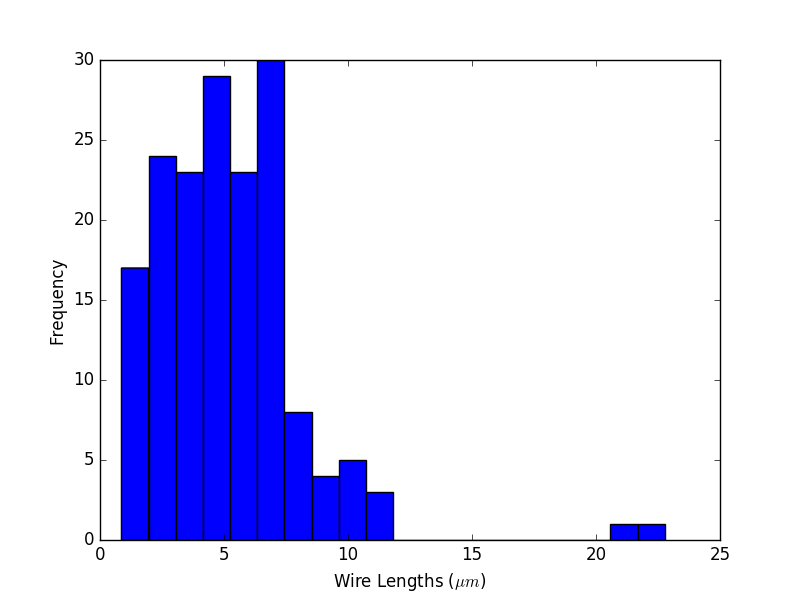
\includegraphics[width=0.7 \columnwidth]{Images/Chapter3/wireLengthDist.png}
\caption{\fontsize{12pt}{11pt}\selectfont Frequency distribution of the wire lengths obtained the digitised NWN shown in Fig. \ref{fig: digitisedNWNs} b). There are a large number of short NWNs with a peak in frequency at around $7 \mu m$ and a quick drop off in wire lengths after this. The mean wire length for this sample is $5.16 \mu m$ and median wire length $4.89 \mu m$.}%
\label{fig: wireLength_Dist}
\end{figure}
\end{comment}


